\documentclass[12pt,a4paper]{article}
\usepackage{times}
\usepackage{durhampaper}
\usepackage{array}
\newcolumntype{P}[1]{>{\centering\arraybackslash}p{#1}}
\usepackage{url}
\usepackage{amsmath}
\usepackage{harvard}
\usepackage[utf8x]{inputenc}
\usepackage{wrapfig}
\usepackage{booktabs}
\usepackage{enumitem}
\usepackage{graphicx}
\usepackage{float}
\usepackage{multirow}
\usepackage{titlesec}
\setcounter{secnumdepth}{4}
\usepackage{cite}
\citationmode{abbr}
\bibliographystyle{plain}
\let\OLDthebibliography\thebibliography
\renewcommand\thebibliography[1]{
	\OLDthebibliography{#1}
	\setlength{\parskip}{0pt}
	\setlength{\itemsep}{0pt plus 0.3ex}
}



\title{An Analysis of Machine Learning and Deep Learning Techniques for Detecting Sarcasm in Text}
\author{} % leave; your name goes into \student{}
\student{Molly Hayward}
\supervisor{Dr Noura Al-Moubayed}
\degree{BSc Computer Science}

\date{}

\begin{document}
	
\maketitle

\begin{abstract}
\\ \noindent \textbf{Context / Background --} 
Sarcasm detection is a relatively new research topic that has recently gained interest due to the increased use of sentiment analysis and social media analytics. Sarcasm is a unique form of language that cannot be interpreted at surface-level, therefore detecting sarcasm proves a significant challenge for traditional sentiment analysers and humans alike. This highlights the scope for innovative machine learning and deep learning solutions to this ill-structured problem.\vspace{5pt}

\noindent \textbf{Aims --} The aim of this project is to contrast the performance of machine learning and deep learning classifiers in order to develop an effective sarcasm detection solution. Furthermore, we investigate to what extent manually extracted sentiment features can be used to enhance machine learning classification in comparison to conventional lexical features. Lastly, we aim to extend our superior binary classification solution in order to highlight tokens that correlate more to sarcastic and non-sarcastic labels.\vspace{5pt}

\noindent \textbf{Method --} We gather two labelled training datasets containing tweets and news headlines, and a third evaluation dataset containing product reviews.\ We apply multiple vectorisation approaches, including a state-of-the-art contextualised embedding approach (ElMo), to transform text into meaningful numerical vectors which are used to train our classifiers.\ An attention mechanism is incorporated into our superior binary classification solution to localise the presence of sarcasm.\vspace{5pt}

\noindent \textbf{Results --} Our bidirectional GRU model trained on the news headlines dataset achieved the highest $F_1$ score of 0.875, although it was less able to generalise to unseen data than our bidirectional LSTM model trained on the Twitter dataset. We integrated our attention mechanism into this bidirectional LSTM model, improving upon our previous $F_1$ score by \_\% and achieving an $F_1$ of 0.862.\vspace{5pt}

%While sentiment features were informative, models trained on these features were unable to rival their deep learning opposition.

\noindent \textbf{Conclusions --} Deep learning models vastly outperform machine learning models in the sarcasm detection task. Furthermore, models trained on ElMo vectors were consistently superior to those trained on all other vector types.

%This section should not be longer than half of a page, and having no more than one or two sentences under each heading is advised. Do not cite references in the abstract.
\end{abstract}\vspace{-10pt}

\begin{keywords}
Machine learning, Deep learning, Sarcasm Detection, Sentiment, Binary Classification, Attention
\end{keywords}\vspace{-10pt}


\section{Introduction}
\noindent Sarcasm is a complex linguistic phenomenon, prevalent in online user-generated content. It is typically used as a form of mockery or humour when expressing an opinion; hence, to interpret sarcastic text literally would be to overlook its implied (usually opposite) meaning. Sarcasm poses a significant challenge within the field of natural language processing as it inverts the sentiment polarity of a positive or negative utterance. This particularly affects sentiment analysis, as this is the task of deducing the sentiment polarity of text - typically whether the author is in favour of, or against, a specific subject. It is increasingly common for organisations to use sentiment analysis to gauge public opinion on their products and services; however, classic sentiment analysers cannot deduce the implicit meaning of sarcastic text and will wrongly classify the author's opinion. Hence, any tool that strives to accurately determine the meaning of user-generated text must be capable of detecting sarcasm. The phenomenon of sentiment incongruity often lies at the heart of sarcasm; hence, advancements in automatic sarcasm detection research have the potential to vastly improve the task of sentiment analysis.\\

\subsection{Problem Background}
\noindent As sarcasm is multi-faceted, detecting it is a unique and interesting challenge.\\



Prior work in the field has primarily focused on overt instances of sarcasm; capturing constrasting positive and negative sentiment phrases \cite{riloff2013sarcasm}, such as \textit{"isn't it great to feel tired?"}, or \textit{"working again tomorrow, yay!"}. However, identifying implicit forms of sarcasm may require knowledge of additional context; as these contextual cues can be more powerful sarcastic indicators than the words themselves. Consider the scenario where a person is congratulated on their hard work, despite the obviousness of them having not worked hard at all. Or perhaps a customer thanking a waiter for the delicious food, despite sending it back to the kitchen. In isolation, the speech is not enough to convey the sarcastic intent; therefore in transcribing this interaction, we lose necessary context and we lose the sarcastic undertones. In the absence of context, we look to more sophisticated deep learning techniques in order to learn the underlying patterns in implicit forms of sarcasm. The first deep learning approach to sarcasm detection was used in \textit{Poria et al. (2017)} \cite{poria2016deeper} to produce state of the art results. \\





However, some forms of sarcasm require additional context; and these contextual cues can be more powerful sarcastic indicators than the words themselves. 


 Overt instances of sarcasm will often utilise contrasting positive and negative sentiment phrases, such as \textit{"isn't it great to feel tired?"}, or \textit{"working again tomorrow, yay!"}.


As such, these instances are simpler to detect than implicit forms of sarcasm; hence, they are the focus of early approaches to sarcasm detection. 

Identifying sarcasm can be a human problem too, as we also struggle to consistently recognise sarcasm; due in part to the lack of an all-encompassing, universal definition. In a 2011 study, Gonz{\'a}lez-Ib{\'a}nez et al. \cite{gonzalez2011identifying} found low agreement rates between human annotators when classifying statements as either sarcastic or non-sarcastic, and in their second study, three annotators unanimously agreed on a label less than 72\% of the time. This suggests that individuals use and perceive sarcasm in different ways; hence, there is no set formula for producing (and therefore identifying) sarcastic text. \\






Across different cultures, sarcasm is used and perceived in unique ways.


Different 
 Additionally, developmental differences such as autism, as well as cultural and societal nuances cause variations in the way different people define and perceive sarcasm.

These factors make sarcasm detection an extremely complex task for both humans and computers. Despite this, \textit{most} humans can recognise sarcastic intent \textit{most} of the time. We strive to replicate this performance, or even perhaps improve upon it, in order to move towards a more concrete definition of what \textit{makes} a statement sarcastic. This highlights the scope for automating this process, and the need for an innovative solution.



\subsection{Research Questions and Objectives}
\noindent The \textbf{research questions} guiding this project are as follows --\\
\indent \textit{- Can handcrafted sentiment features improve sarcasm predictions?}\\ 
\indent \textit{- Do deep learning techniques perform better than machine learning approaches?}\\ 
\indent \textit{- Can a custom model identify which linguistic cues correlate more to sarcastic labels?}\\

\noindent The following objectives are designed to address these specific research questions, and are divided into three categories depending on their priority level and difficulty.\\

\noindent The \textbf{minimum} objectives of this project were to evaluate and clean high-quality datasets, and to employ machine learning models in order to evaluate their performance on our chosen datasets. To fulfil these objectives we gathered two large balanced datasets containing Twitter data and news headlines; as well a small unbalanced corpus of product reviews. Gathering data from multiple online sources enabled us to take into account the versatility of sarcasm usage online. After implementing five machine learning classifiers, we found that our logistic regression model performed best for both datasets, achieving  $F_{1}$ scores of 0.851 and 0.790.\ The purpose of this objective was to establish a baseline against which to compare the performance of our deep learning classifiers.

The \textbf{intermediate} objectives of this project are to experiment with and evaluate deep learning models on the chosen datasets, and to determine which is the best performing solution. Additionally, we evaluate the model against unseen data. This is achieved by ...

The \textbf{advanced} objectives of this project are to implement an attention-based neural network in order to identify words that correlate more to sarcastic labels, in order to produce a visualisation of attention words. We implement a custom attention layer using keras, and apply our trained model to a number of sentences to illustrate its effectiveness.

This is achieved by...




%This section briefly introduces the general project background, the research question you are addressing, and the project objectives.  It should be between 2 to 3 pages in length.\\%

\section{Related Work}
\noindent In this section, we report on the architectural design of solutions used specifically in sarcasm detection research, as well as techniques that have seen success in other natural language processing (NLP) classification tasks. Oftentimes, sarcasm detection is treated as a binary classification problem, in which text is grouped into two categories - sarcastic and non-sarcastic. It is otherwise treated as a multi-class problem where the extent to which a statement is sarcastic is ranked on a discrete scale, e.g. 1 to 5. In similar studies, the terms irony and sarcasm are used synonymously \cite{tsur2010icwsm}, although their definitions differ slightly (\textit{table 1}). Both definitions capture the humourous intent in both sarcasm and irony, however sarcasm includes the potential for mockery and criticism - often present in opinion-based content such as product reviews.\vspace{-2pt}

\begin{center}
	\textbf{Table 1}: Definitions of Irony and Sarcasm\vspace{-5pt}
\end{center}
\begin{center}
	\begin{tabular}{p{1.5cm}p{13.2cm}}
		\hline
		\textbf{Term} & \textbf{Definition}\\
		\hline\hline
		Irony & A subtle form of humour which involves saying things that you do not mean. \footnotemark[1]\\
		\hline
		Sarcasm & Speech or writing which actually means the opposite of what it seems to say, usually intended to mock or insult. \footnotemark[2]\\
		\hline
	\end{tabular}\\
\end{center}\vspace{-10pt}
\footnotetext[1]{https://www.collinsdictionary.com/dictionary/english/irony}
\footnotetext[2]{https://www.collinsdictionary.com/dictionary/english/sarcasm}

\subsection{Rule-based Classifiers}\vspace{-10pt}
\noindent A number of na\"{i}ve approaches have been used in previous research, where text is classified based on a set of linguistic rules. Bharti et al. (2015) \cite{bharti2015parsing} proposed two rule-based approaches - one approach (IWS) classifies tweets that begin with injerjections, such as \textit{"wow"} and \textit{"yay"}, as sarcastic, and the other uses a parsing based lexical generation algorithm (PBLGA) to recognise sentiment-bearing situation phrases juxtaposed with contrasting sentiment phrases. When tested on 1500 tweets containing \#sarcasm, the IWS and PBLGA approaches yielded $F_1$ scores of 0.90 and 0.84, respectively. An earlier example of a rule-based approach is displayed in Maynard and Greenwood (2014) \cite{maynard2014cares}. They proposed that the sentiment contained in hashtags can indicate the presence of sarcasm in tweets, such as \#notreally in the example \textit{"I love doing the washing-up \#notreally"}. They used a rule-based approach where tweets are labelled as sarcastic if their sentiment contradicts the sentiment of the hashtag, reporting an $F_{1}$ score of 0.91. 

Rule-based classifiers can perform well if their rule-sets are tailored to specific datasets - however, they cannot generalise effectively to data that is structurally different, hence they are considered  primitive when compared to their modern, deep learning counterparts.

\subsection{Machine Learning Classifiers}\vspace{-10pt}
\noindent Machine learning algorithms do not rely upon a static linguistic rule-set and can instead learn the underlying patterns associated with each class, allowing them to accurately classify unseen data.\ Previous research predominantly focuses on the use of tree-based classifiers, support-vector machines (SVM) and logistic regression models, although not all approaches fit neatly into these categories. For instance, Tsur et al.\ (2010) \cite{tsur2010icwsm} proposed a novel semi-supervised algorithm, \textit{SASI}, for sarcasm identification; trained on a small balanced seed of 160 human-annotated product reviews from a corpus of 66000. In order to mimic the ambiguous and spectral nature of sarcasm, a discrete score between 1 (non-sarcastic) and 5 (definitely sarcastic) is assigned to each sentence; scores of 3 and higher indicate sarcasm. Syntactic and pattern-based features are extracted and fed to a classifier which utilises a strategy similar to K-Nearest Neighbours (kNN), whereby a sarcasm score is assigned to an unseen vector based upon the weighted average of the k closest vectors from the training set. They reported an $F_{1}$ score of 82.7\% on the binary classification task.

As one of the first studies to consider sentiment features, Riloff et al. (2013) \cite{riloff2013sarcasm} describes sarcasm as a contrast between positive sentiment (e.g.\ \textit{"i love"}), in reference to a negative situation (e.g.\ \textit{"being ignored"}). They use a bootstrapping algorithm to extract positive verb phrases and negative situation phrases from a Twitter corpus and used these to train a hybrid model consisting of a SVM and a contrast method which classifies text as sarcastic if a postive sentiment phrase precedes a negative situation. This yielded an $F_1$ score of 51\%. Gonz{\'a}lez-Ib{\'a}nez et al. (2011) \cite{gonzalez2011identifying} also considered unique miscellaneous features, including lexical (e.g. unigrams) and pragmatic (e.g. emoticons) features. They trained an SVM with sequential minimal optimisation and a logistic regression model, achieving 71\% accuracy using an SVM trained on unigrams. Pt{\'a}{\v{c}ek et al. (2014)} \cite{ptavcek2014sarcasm} also used a support-vector machine, performing classification on balanced and inbalanced datasets.

Reyes et al. (2013) \cite{reyes2013multidimensional} used a na\"{i}ve bayes and decision trees algorithm in order to detect irony which is closely related to sarcasm. They experimented with balanced and unbalanced distributions (25\% ironic tweets and 75\% other), achieving an F-score of 0.72 on the balanced distribution, dropping to 0.53 for the inbalanced distribution. In a similar vein, Barbieri et al. (2014) \cite{barbieri2014modelling} used random forest and decision tree classifiers, also for the detection of irony. They used six types of features in order to represent tweets, and recorded results over three categories of training data - education, humor and politics.



\subsection{Deep-Learning Classifiers}\vspace{-10pt}
Deep neural networks (DNNs) are increasingly being used in text classification tasks \cite{zhang2015character, poria2016deeper}. Though there are many forms of DNN, two commonly used architectures are Recurrent Neural Networks (RNNs) and Convolutional Neural Networks (CNNs). Oftentimes, deep neural networks require a lot more training data than machine learning algorithms, but have been shown to produce state-of-the-art results in several domains. If the training data is high-quality and plentiful, then the model can begin to make accurate predictions. 

%https://arxiv.org/pdf/1703.03091.pdf



 A similar technique was applied in \textit{Ghosh et al. 2018)} \cite{ghosh2018sarcasm} where they concluded that emoticons such as ':)' and interjections e.g. "ah", "hmm" correspond with highly weighted sentences. Gated Recurrent Units (GRUs) are another type of RNN used to overcome the vanishing gradient problem.  \textit{Zhang et al. (2016)} \cite{zhang2016tweet} used a bidirectional gated RNN to capture local information in tweets, as well as a pooling neural network to extract context from historic tweets, achieving 78.55\% accuracy.

Convolutional Neural Networks allow us to extract higher-level features, and they are based on the mathematical operation of convolution. \textit{Zhang et al. (2015)}  \cite{zhang2015character} explored the used of character-level convolutional neural networks for text classification. This network consists of 6 convolutional layers and 3 fully-connected layers. They found that it showed better peformance on raw texts such as an Amazon product review corpus.

In \textit{Poria et al. (2017)} \cite{poria2016deeper}, cited as the first study to use deep learning for sarcasm detection.


CNNs have been previously used in sarcasm detection. For example, \textit{Poria et al. (2017)} \cite{poria2016deeper} describes a convolutional neural network (CNN) for sarcasm detection. \\

\subsection{Attention}\vspace{-10pt}
One particularly interesting technique is the \textit{Hierarchical Attention Network (HAN)} defined in Yang et al. (2016) \cite{yang2016hierarchical} - an attention-based LSTM. The intuition is that certain words and sentences in a document contribute more to its overall meaning, and this is highly context dependent. They included one attention mechanism at word-level and another at sentence-level, and this allowed them to determine which words and phrases correlate more to certain labels. Using a similar approach in the domain of sarcasm may allow me to highlight the attention-words that are strongly influence the level of sarcasm.


%In Yang et al. 2016, they used two sentence-level and word-level attention


%Additionally, we use a bidirectional model so as to account for both the left and right contexts of words. 

%We use a bidirectional GRU and concatenate the output sequences from both GRUs. 
%This paper considers that documents have a hierarchical structure

%The attention mechnism has played a fundamental role in recent deep learning research, fuelling powerful language models such as BERT. 

%An Attention mechanism attributes more importance to a subset of the input words.

%Bahdanau et al. (2015) suggested that a context vector takes into account all of the input words, assigning relative importance to some more than others.

%This section presents a survey of existing work on the problems that this project addresses.  it should be between 2 to 4 pages in length.  The rest of this section shows the formats of subsections as well as some general formatting information for tables, figures, references and equations. Note that the whole report, including the references, should not be longer than 20 pages in length.  The system will not accept any report longer than 20 pages.  It should be noted that not all the details of the work carried out in the project can be represented in 20 pages.  It is therefore vital that the Project Log book be kept up to date as this will be used as supplementary material when the project paper is marked.  There should be between 10 and 20 referenced papers---references to Web based pages should be less than 10\%.



%The font used for the main text should be Times New Roman (Times) and the font size should be 12.  The first line of all paragraphs should be indented by 0.25in, except for the first paragraph of each section, subsection, subsubsection etc. (the paragraph immediately after the header) where no indentation is needed.


%In general, figures and tables should not appear before they are cited.  Place figure captions below the figures; place table titles above the tables.  If your figure has two parts, for example, include the labels ``(a)'' and ``(b)'' as part of the artwork.  Please verify that figures and tables you mention in the text actually exist.  make sure that all tables and figures are numbered as shown in Table \ref{units} and Figure 1.
%sort out your own preferred means of inserting figures


%The list of cited references should appear at the end of the report, ordered alphabetically by the surnames of the first authors.  References cited in the main text should use Harvard (author, date) format.  When citing a section in a book, please give the relevant page numbers, as in \cite[p293]{budgen}.  When citing, where there are either one or two authors, use the names, but if there are more than two, give the first one and use ``et al.'' as in  , except where this would be ambiguous, in which case use all author names.


%You need to give all authors' names in each reference.  Do not use ``et al.'' unless there are more than five authors.  Papers that have not been published should be cited as ``unpublished'' \cite{euther}.  Papers that have been submitted or accepted for publication should be cited as ``submitted for publication'' as in \cite{futher} .  You can also cite using just the year when the author's name appears in the text, as in ``but according to Futher \citeyear{futher}, we \dots''.  Where an authors has more than one publication in a year, add `a', `b' etc. after the year.

\section{Solution}
\noindent This project addresses a binary classification problem, aiming to determine if an unseen snippet of text is sarcastic or non-sarcastic. Our sarcasm detection tool employs trained classification models which form  predictions based on knowledge gained from features encountered during training. Developing highly accurate classification models remains the greatest challenge in this project, therefore it is the central focus of our solution. Model peformance is strongly dependent on the data pre-processing and feature extraction techniques employed, as well as the choice of model architecture and training procedures. 

In our solution, high quality datasets are first collected and pre-processed. During feature extraction, the textual training data is transformed into numerical vectors and these features are used to train a classification model. The trained classifier is then carefully evaluated in order to account for potential overfitting. The following figure outlines the model pipeline, and each of these stages are further addressed in the remaining sections.

\begin{center}
	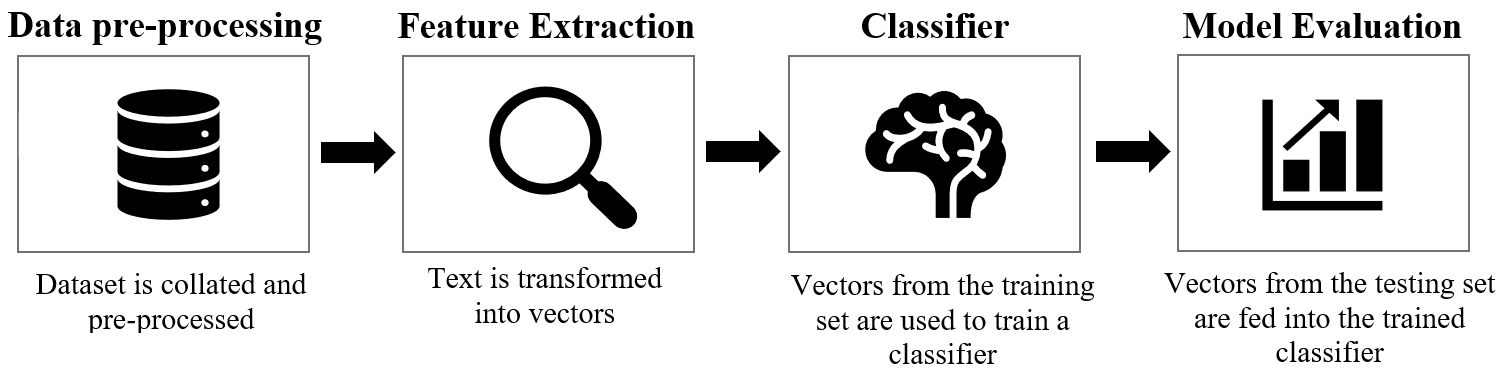
\includegraphics[width=0.8\textwidth]{Images/modelpipeline2.png}
	\label{Model Pipeline}\\
	\textbf{Figure 1:} Overview of the solution
\end{center}

\subsection{Implementation Tools}\vspace{-4.2pt}
\noindent This project is majoritively written in Python, as it has an abundance of open-source libraries well-suited to machine learning and deep learning tasks. Furthermore, Python is very readable, making it easy for others to test and reproduce results. We use pandas for manipulating our datasets, as it provides functionality for applying functions to all instances at the same time, and harness the built-in functionality from SpaCy to clean and tokenise our data. In terms of \textit{classification}, we implement most of the machine learning architectures using scikit-learn - an open-source machine learning library. For constructing deep learning models, we use keras as its modular structure allows for extensive experimentation and tweaking of model architectures.

\subsection{Datasets}
\vspace{-4.2pt}\noindent We utilise three publically available datasets and provide a statistical analysis of their properties in \textit{table 2}. This includes the number of instances in the dataset, the average number of tokens per instance and a benchmark score where the dataset was used in the original paper to train one or more classifiers. This data is collected from multiple domains and online platforms, including Twitter, Amazon, and online news outlets; providing broad coverage of sarcasm usage in both formal and informal media. We use our News Headlines and Twitter datasets for training, and reserve our Amazon review corpus for cross-dataset evaluation.\vspace{-5pt}

\begin{enumerate}[leftmargin=0cm]
	\item \textbf{News Headlines} - \textit{Misra et al.\ (2019)} \cite{misra2019sarcasm} collected thousands of news headlines from two sources - \textit{The Onion} \footnotemark[3]\footnotetext[3]{www.theonion.com} (renowned for posting satiricial news) and \textit{The Huffington Post} \footnotemark[4]\footnotetext[4]{www.huffpost.com}. They utilised a hybrid neural network architecture and achieved a classification \textit{accuracy} of 0.897.\vspace{-5pt}
	
	\item \textbf{Twitter Data} - Collated in \textit{Pt\'a\v{c}ek et al.\ (2014)} \cite{ptavcek2014sarcasm}, we use the balanced dataset of 100000 English tweets. Of this original corpus, 17.28\% of tweets remain available to access on Twitter, therefore all others are omitted from the compiled dataset. Sarcastic instances are tweets that include \textit{\#sarcasm}, and non-sarcastic instances are selected arbitrarily from the set of all other tweets. Pt\'a\v{c}ek et al.\ (2014) \cite{ptavcek2014sarcasm} achieved an $F_{1}$ score of 0.947.\vspace{-5pt}
	
	\item \textbf{Amazon Reviews} - \textit{Filatova (2012)} \cite{filatova2012irony} used crowdsourcing to collect Amazon reviews, human-labelled by 5 annotators. This dataset was not used by its compilers for classification, hence there is no score available for comparison.
\end{enumerate}

% For example, we avoid using datasets containing tweet ids, whereby the original tweet must be scraped using the Twitter API. A small portion of the original tweets are no longer available on twitter, therefore this does not make for a fair comparison between our results and the results of the source study.


\begin{center}
	\textbf{Table 2}: Statistical breakdown of the datasets used in this project \\
	\vspace{3pt}
	\begin{tabular}{P{3cm}P{1cm}P{2.4cm}P{2.2cm}P{2.1cm}P{3.25cm}}
		\hline
		\textbf{Dataset} & \textbf{Usage}& \textbf{Dataset Size} & \textbf{Composition}* & \textbf{Avg. tokens} & \textbf{Benchmark Score}\vspace{1pt}\\
		\hline
		News Headlines & Training & 28619 & \begin{tabular}{c@{}@{}@{}} pos: 47.6\% \\ neg: 52.4\% \end{tabular} &  11.2 & 0.897\\
		\hline
		Twitter Data & Training & 17280 & \begin{tabular}{c@{}@{}@{}} pos: 50.4\% \\ neg: 49.6\% \end{tabular} &  19.8 & 0.947 \\
		\midrule
		Amazon Reviews & Testing & 1254 & \begin{tabular}{c@{}@{}@{}} pos: 34.9\% \\ neg: 65.1\% \end{tabular} &  276.4 & N/A \\
		\hline
	\end{tabular}
\end{center}
\vspace{-7pt}
*\textit{pos} indicates positive instances (sarcastic) and \textit{neg} indicates negative instances (non-sarcastic)\\

\noindent The training datasets used in this project are large enough to provide a representative view of their respective data sources, without exceeding our computational resources. Furthermore, they are approximately balanced; despite the fact that sarcasm is used infrequently in real-life. On an unbalanced dataset, a classifier can achieve high accuracy simply by annotating each data instance with the majority class label.\ As most machine learning algorithms are designed to optimise overall accuracy, it is important to provide them with approximately equal amounts of both sarcastic and non-sarcastic data, to prevent them from overfitting to either class.


\subsection{Data Pre-Processing}
\vspace{-4.2pt}
\noindent Datasets of user-generated content are inherently noisy and ill-structured, as users are free to include spelling errors and inconsistent capitalisation. Pre-processing is necessary for removing as much of this noise as possible to reduce sparsity in the feature space; although, we must be careful not to remove useful features.

On Twitter, users can include hyperlinks and references to other users in their tweets; however, this can be a source of noise in the dataset therefore we remove them using regular expressions. In \textit{Pt{\'a}{\v{c}ek et al. (2014)}} \cite{ptavcek2014sarcasm}, hashtags are removed in pre-processing. However, \textit{Liebrecht et al. (2013)} \cite{liebrecht2013perfect} showed that the sentiment contained in hashtags can be used to indicate sarcasm, such as the use of \#not to suggest insincerity. In the simplest case, single-word hashtags can be included simply by removing the \# symbol, however multi-word hashtags must first be parsed to separate the tokens. As this is beyond the scope of this project, we remove all hashtags with the exception of \textit{\#not} (which we substitute with \textit{not}).

Punctuation is removed and text is transformed to lowercase in order to reduce sparsity induced by the optional inclusion of punctuation and variations in letter capitalisation. This ensures that are fewer representations of the same word, as tokens such as \textit{'CAN'T'}, \textit{'can't'}, and \textit{'Cant'} are all mapped to the same single token - 'cant'. However, punctuation and capitalisation can be used for emphasis, which may in turn be indicative of sarcasm. Hence, we re-introduce this meaning in the form of additional lexical features using a procedure outlined in the feature extraction section. Finally, we remove numbers and stopwords, such as \textit{'the'}, \textit{'in'} and \textit{'an'}, as they provide little additional meaning to a sentence despite the number of times they occur.

\begin{center}
	\textbf{Table 3}:  Proportion of tokens represented in the GloVe dictionary\\
	\vspace{4pt}
	\begin{tabular}{p{3cm}||p{3cm}p{3cm}}
		\hline
		\textbf{Dataset} & \textbf{Original data} & \textbf{Processed data}\\
		\hline
		News Headlines & \hspace{20pt}97.71\% & \hspace{20pt}97.71\%\\
		\hline
		Twitter Data & \hspace{20pt}89.62\% & \hspace{20pt}96.43\%\\
		\hline
		Amazon Reviews & \hspace{20pt}83.17\% & \hspace{20pt}98.22\%\\
		\hline
	\end{tabular}\\
\end{center}

\noindent Figure \_ shows the proportion of GloVe-representable tokens before and after processing, where the same processing techniques are applied to each dataset. GloVe is a word-embedding technique, detailed in the feature extraction section, where tokens are encoded as pre-computed numerical vectors. We use the number of tokens represented in the GloVe dictionary (containing 27 billion tokens) as a measure of quality, as uncommon or ill-formed tokens are ommitted from this dictionary. The quality of the Amazon and Twitter data vastly improved after processing, however the quality of the news headlines corpus remained consistent as the original data is written formally and in lowercase.

%This section presents the solutions to the problems in detail.  The design and implementation details should all be placed in this section.  You may create a number of subsections, each focussing on one issue.  

%This section should be between 4 to 7 pages in length.

\subsection{Feature Extraction}
\vspace{-4.2pt}
\noindent Extracting meaningful data from large corpora is vital for enabling classifiers to make high-quality predictions. As such, it follows that in the context of natural language processing, feature extraction techniques should encode the underlying semantics of text into the numeric vectors they produce. We produce our dominant features using established vectorisation techniques such as GloVe \cite{pennington2014glove} and ElMo \cite{peters2018deep}. However, we also experiment with a number of custom features in combination with our main features, generated using the procedures outlined in \textit{section D.2}. \vspace{-4.2pt}

\subsubsection{Main Features}
\noindent \textbf{Traditional Approaches --} As our least advanced feature extraction techniques, \textit{Bag of Words (BOW)} and \textit{Term Frequency-Inverse document frequency (TF-IDF)} \cite{robertson1976relevance} are used as a baseline against which to compare more advanced approaches. In BOW, text is encoded as a single vector containing a count of the number of occurrences of each word. TF-IDF extends the BOW model by providing each word with a score that reflects its importance based upon its frequency within the document. These approaches create sparse inefficient representations, where each vector is the size of the vocabulary. Additionally, vectors produced in this way do not preserve the context within which words are found, although sarcasm is a highly contextual phenomenon.\\

\noindent \textbf{Word Embedding --} Introduced in Mikolov et al.\ (2013a) \cite{mikolov2013efficient}, \textit{Word2Vec} describes a group of related models that were the first to produce high-quality vector representations of words, known as word embeddings. Word2Vec consists of a shallow (two-layer) neural network that takes a large corpus and produces lower-dimensional vectors than the sparse representations generated by BOW and TF-IDF; however, intrinsic statistical properties of the training corpus, which were key to earlier techniques, are neglected, therefore global patterns may be overlooked. To mitigate this, we use the \textit{GloVe} \cite{pennington2014glove} approach, which generates word embeddings by constructing an explicit word co-occurrence matrix for the entire corpus. Word embeddings appear in a high-dimensional vector space, whereby words that share a similar context are clustered together.\\

\begin{minipage}{0.3\textwidth}
	\vspace{-10pt}
	\begin{center}
		\hspace{-1cm}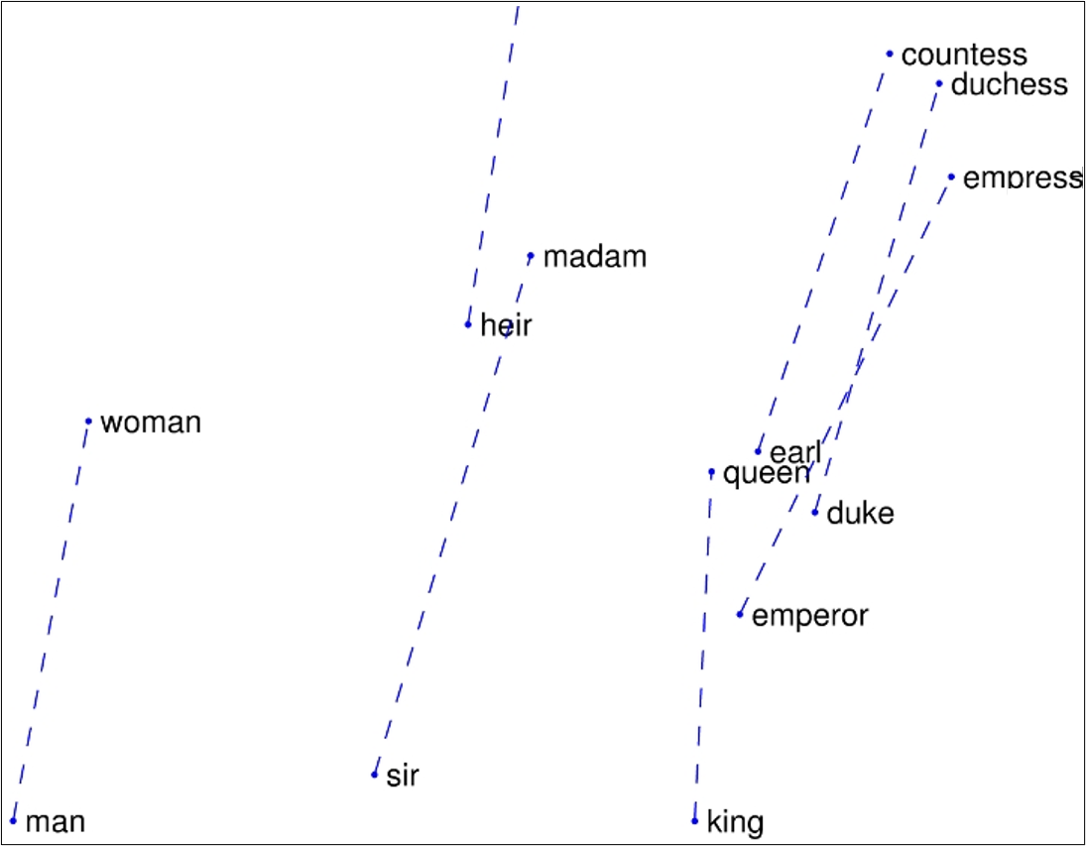
\includegraphics[width=1.05\textwidth]{Images/outside1.png}\\
		\hspace{-1cm}\textbf{Figure 2:} GloVe substructure\footnotemark[5]\\
		\label{Glove Model}
	\end{center}
\end{minipage} \hfill
\begin{minipage}{0.66\textwidth}
	 GloVe is able to preserve the semantic relationships between words, even constructing analogies by composing vectors e.g.\ $king - man + woman ≈ queen$. Likewise, it captures syntactic regularities such as the singular to plural relationship e.g.\ $cars - car ≈ apples - apple$. GloVe is used in this project to produce word embeddings for each corpus, however it does not accommodate polysemy, which describes the co-existence of alternative meanings for the same word, and cannot generalise to words that were not specifically included in the training set.\\
\end{minipage}\\
\footnotetext[5]{https://nlp.stanford.edu/projects/glove/}

%To mitigate this, we use the \textit{GloVe} \cite{pennington2014glove} approach, which generates word embeddings by constructing an explicit word co-occurrence matrix for the entire corpus. Word embeddings appear in a high-dimensional vector space, whereby words that share a similar context are clustered together. GloVe is able to preserve the semantic relationships between words, even constructing analogies by composing vectors e.g.\ king - man + woman ≈ queen. Likewise, it captures syntactic regularities such as the singular to plural relationship e.g.\ cars - car ≈ apples - apple. GloVe is used in this project to produce word embeddings for each corpus, however it does not accommodate polysemy, which describes the co-existence of alternative meanings for the same word, and cannot generalise to words that were not specifically included in the training set.\\

\noindent \textbf{Contextualised Word Embedding --} Peters et al\ (2018) \cite{peters2018deep} introduced the \textit{ELMo} model, and showed that ELMo markedly improved the state-of-the-art in a number of NLP tasks.\\\vspace{-10pt}

\begin{minipage}{0.3\textwidth}
	 	\begin{center}
		\hspace{-1.5cm}\includegraphics[width=1.2\textwidth]{Images/elmo_diagram2.png}\\
		\hspace{-1cm}\textbf{Figure 3:} ElMo model pipeline\\
		\label{ElMo Model}
	\end{center}
\end{minipage} \hfill
\begin{minipage}{0.66\textwidth}
	  ELMo utilises a bi-directional LSTM \textit{(long short-term memory)} model, concatenating the left-to-right and right-to-left LSTM in order to produce deep contextualised word representations. They are character based, therefore robust representations can be constructed for out-of-vocabulary tokens. However, rather than 'looking-up' pre-computed embeddings, ELMo generates them dynamically. Hence, it can disambiguate the sense of a word given the context in which it was found. These state-of-the-art contextualised embeddings are used in this project as the most advanced method of feature extraction.
\end{minipage}\\

\subsubsection{Miscellaneous Features}
We consider miscellaneous features as well as those produced by the aforementioned techniques - including lexical (punctuation) features, topic features and sentiment features. We focus specifically on the effects of incorporating our \textit{novel sentiment features} in comparison to incorporating more conventional punctuation and topic features. We produce low-dimensional feature vectors for each of our datasets, concatenating those that are shown to improve classifcation scores with existing vectors.\\\vspace{-5pt}

\noindent \textbf{1. Punctuation features --} We extract punctuation features following the procedure outlined in Tsur et al. (2010) \cite{tsur2010icwsm}. Five lexical features are combined to produce a $ 1 \times 5 $ dimensional vector for each text snippet, including the length of the snippet in tokens, as well as the number of: "!" characters, "?" characters, quotations and tokens that include at least one capitalised character. These features are normalised by dividing them by the (maximal observed value $ \cdot $ average maximal value of remaining feature groups).\\\vspace{-5pt}

%\begin{enumerate}
%	\item "!" characters\vspace{-10pt}
%	\item "?" characters\vspace{-10pt}
%	\item Quotations\vspace{-10pt}
%	\item Tokens that include at least one capitalised character
%\end{enumerate}

\noindent \textbf{2. Topic features --} We use Latent Dirichlet Allocation (LDA) to perform topic modelling - this is an unsupervised machine learning technique where a fixed number of abstract "topics" are identified in a corpus. Each instance in a dataset is represented as the distribution of its topics, relative to the topics in the global dataset. The intuition is that positive and negative instances may each contain their own distinct assortment of topics, thereby informing future predictions on unseen sarcastic and non-sarcastic data.\\\vspace{-5pt}

\noindent \textbf{3. Sentiment features --} We produce sentiment features using the state-of-the-art \textit{SentimentAnnotator} \cite{socher2013recursive} by Stanford CoreNLP \cite{manning2014stanford} which assigns a discrete sentiment label to text, where 0 is very negative and 4 is very positive.\\\vspace{-5pt}

\hspace{-15pt}\begin{minipage}{0.55\textwidth}
	\textit{Example: "i love when my train is late"}\vspace{-15pt}
	\begin{center}	
		\begin{tabular}{|m{1.8cm}||m{0.4cm}m{0.6cm}m{0.75cm}m{0.4cm}m{0.7cm}m{0.2cm}m{0.6cm}|}
			\hline 
			\textbf{Tokens} & \textbf{i} & \textbf{love} & \textbf{when} & \textbf{my} & \textbf{train} & \textbf{is} & \textbf{late}\\ 
			\hline 
			Sentiment & 2 & 4 & 2 & 2 & 2 & 2 & 1\\ 
			\hline 
		\end{tabular}
		\vspace{5pt}
		
		\begin{tabular}{|p{1.8cm}||p{0.9cm}|p{0.9cm}|p{0.9cm}|p{0.9cm}|p{0.9cm}|} 
			\hline 
			\textbf{Sentiment} & \textbf{0} & \textbf{1} & \textbf{2} & \textbf{3} & \textbf{4}\\ 
			\hline 
			Frequency & 0 & 1 & 6 & 0 & 1\\ 
			Proportion & 0 & 0.125 & 0.750 & 0 & 0.125\\
			\hline  
		\end{tabular}
	\end{center}
	Overall sentiment: 3.0\\
	Feature vector: [0.0, 0.125, 0.750, 0.0, 0.125, 3.0]\\
\end{minipage}
\hspace{15pt}\begin{minipage}{0.4\textwidth}
	\vspace{-5pt}
	For each instance in the dataset, we collect the sentiment values for each of the individual tokens, as well as the overall sentiment of the snippet. We contruct $ 1 \times 6 $ dimensional feature vectors, where values 0 - 4 show the distribution of sentiment classes for tokens in the snippet, and value 5 shows the overall sentiment label.\\
\end{minipage}



\subsection{Binary Classification}\vspace{-5pt}
\noindent In this section, we describe the machine learning and deep learning classifiers used in this project. These algorithms are trained on a set of rich features. For example, our machine learning classifiers are trained on Bag of Words, TF-IDF, GloVe and ElMo vectors, and we experiment with concatenating miscellaneous features where they have been proven to be informative in our binary classification task.\ We train each deep learning model on GloVe and ElMo vectors only, as it is computationally intractable to train neural networks on high-dimensional sparse features.\vspace{-5pt}

\subsubsection{Machine Learning Models}
We experiment with five candidate machine learning classifiers, evaluating each of them when trained on four types of features. Each of these supervised models performs binary classification, where unseen samples are predicted to be sarcastic or non-sarcastic. Brief descriptions of the models are provided below in the context of our specific binary classification problem. \vspace{-3pt}

\begin{enumerate}
	\item \textbf{Na\"{i}ve Bayes Classifier --} A group of probabilistic models that use Bayes theorem to make predictions; variations include Multinomial, Bernoulli and Gaussian Na\"{i}ve Bayes. The na\"{i}ve assumption that all features are independent of one another allows an estimate of ${P(Sarcastic \text{ }| \text{ }x)}$ (i.e. probability that a statement is sarcastic, given its feature vector, x) to be made using Bayes theorem.\vspace{-3pt}
	
	\item \textbf{K-Nearest Neighbours (KNN) --} A non-parametric model which uses lazy learning at the time of prediction. An unseen sample is assigned the majority class label amongst its k nearest neighbours, where k is a hyperparameter to be finetuned. We found that k=5 achieved the optimal balance between the computational cost of a large number of neighbours and increased noise and bias associated with small values of k.\vspace{-3pt}
	
	\item \textbf{Support-Vector Machine (SVM) --} Uses a kernel function to draw a hyperplane which divides a feature space into two subspaces. Features at the shortest euclidean distance (\textit{margin}) to the hyperplane are known as support-vectors, and their distance from the hyperplane is maximised to create a decisive boundary between the sarcastic and non-sarcastic data. Our SVM uses a linear kernel as this model performed better than the SVM with radial basis function (RBF) kernel.\vspace{-3pt}

	\item \textbf{Logistic Regression --} Models a binary dependent variable by finding a relationship between features and the likelihood that they belong to either class. It is a more advanced approach than linear regression, which aims to model data using a linear equation.\vspace{-3pt}

	\item \textbf{Random Forest Classifier --}
	An ensemble learning method which fits a number of decision trees on subsamples of the training set. The decision trees produce class predictions which are condensed into a single prediction by means of voting. As they are largely independent of one another, this low correlation allows them to produce collective predictions that outperform their individual predictions.
\end{enumerate}


\subsubsection{Deep Learning Models}
Deep learning classifiers do not require the  hand-crafted features used in supervised classifiers, and are instead capable of learning higher-level features from dense vectors such as ElMo and GloVe. We focus on two categories of neural networks - Convolutional Neural Networks (CNN) and Recurrent Neural Networks (RNN). While it is beyond the scope of this paper to describe in detail the concepts involved in CNNs and RNNs, we provide a brief explanation below. As we are performing binary classification, we use the Binary Cross-Entropy loss function.\\\vspace{-5pt}

\noindent \textbf{Convolutional Neural Networks (CNN)}\cite{lecun1998gradient} were popularised for their applications in computer vision and were designed to be used with image data \cite{krizhevsky2012imagenet}; however, they can be adapted for text-based classification tasks by replicating the two-dimensional structure of images (\textit{figure 4}).\vspace{-5pt}
%CNNs include a variable number of convolutional layers with non-linear activations - they typically have fewer layers than other neural networks, where each layer applies dfferent filters and combines their result. 

\hspace{-20pt}\begin{minipage}{0.35\textwidth}
	\vspace{-5pt}\begin{figure}[H]
		\begin{center}
			$
			\begin{bmatrix}
			w_{1,1} & w_{1,2} & ... & w_{1,N}\\
			\vdots & \vdots & \vdots & \vdots \\
			w_{M, 1} & w_{M, 2} & ... & w_{M, N} \\
			\end{bmatrix}
			$\vspace{5pt}
			\textbf{Figure 4}: $m \times n$ feature vector\\
		\end{center}
	\end{figure}
\end{minipage} \hfill
\begin{minipage}{0.62\textwidth}
	\vspace{-8pt}
	To create input features for the CNN, each token in a sentence is represented independently by a fixed-size n-dimensional vector; as such, the sentence is represented by an $m \times n$ vector of feature weights, where m is the number of tokens in the sentence.
\end{minipage}\vspace{-5pt}

%Convolutional layers compute the dot product of a kernel vector of k weights with k rows in the feature vector (representing k-tokens in the input sentence), producing a new sequence of features.
\noindent The characterising feature of a CNN is the convolutional layer, where filters are applied to feature vectors using the mathematical operation of convolution, and a max pooling operation is applied over each resulting feature map. Tokens in a sentence occur on a time axis, as the order that the tokens appear in gives rise to their meaning; hence, the filter slides downwards over the rows of the vector (\textit{maximum pooling over time}) to produce a single output value. This is especially useful for classification tasks, where the desired output is a fixed-sized vector representing a class. Due to the high speed of the convolution operation, many convolutional layers can be used in a single network without excessivly slowing the training process.

We implement two convolutional neural networks and present their architectures in \textit{figure 5}. We refer to one as a simple CNN as it contains only one convolutional layer, and to the other as a deep CNN as we incorporate three convolutional layers. With over 1.7 million trainable parameters, our deep CNN is more computationally complex and is slower to train than our simple CNN, which contains approximately 140 thousand trainable parameters. Both networks take an $N \times L$-dimensonal vector, where N is the length of each token vector, and L is the number of tokens in the snippet.\vspace{-16pt}

\hspace{-20pt}\begin{minipage}{0.4\textwidth}
	\begin{figure}[H]
		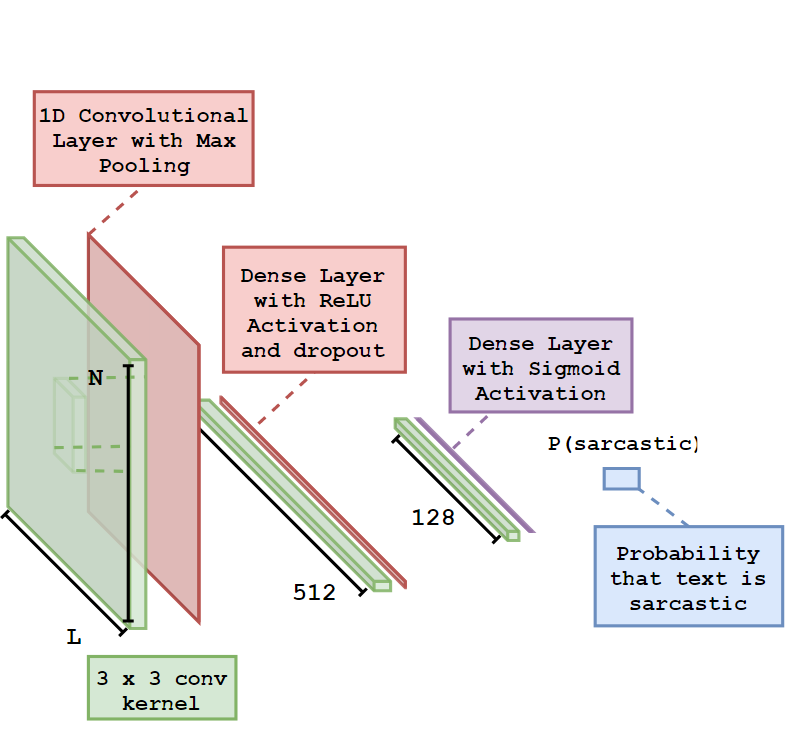
\includegraphics[width=1\textwidth]{Images/CNNarchNew.png}
		\centering\textbf{(a)} Simple CNN Architecture\\
	\end{figure}
\end{minipage}
\hspace{10pt}
\begin{minipage}{0.6\textwidth}
	\begin{figure}[H]
		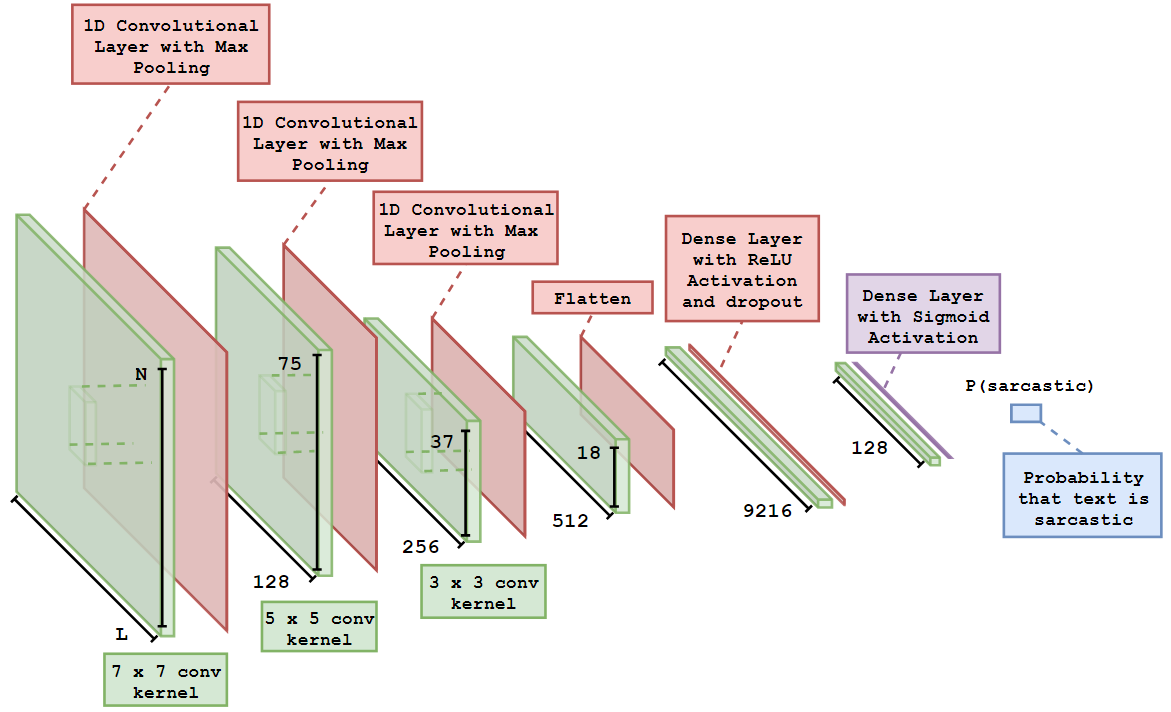
\includegraphics[width=0.97\textwidth]{Images/DCNNarchNew.png}
		\centering\textbf{(b)} Deep CNN Architecture\\
	\end{figure}
\end{minipage}\\\vspace{-7pt}

\begin{center}
	\textbf{Figure 5}: Illustration of Convolutional Neural Network Architectures\\
\end{center}


\noindent \textbf{Recurrent Neural Networks (RNN)} use feedback loops to process sequential data, creating a form of \textit{memory} that allows information to persist in the network. RNNs maintain an additional hidden state, \textit{h}, containing its own set of biases and weights.\vspace{5pt}

\hspace{-20pt}\begin{minipage}{0.6\textwidth}	
	 We can unroll this loop (\textit{figure 6}) to reveal how outputs from previous time steps continue to propagate through the network.\ RNNs take an input sequence, denoted by \textit{x}, and return an output sequence, denoted by \textit{y}, which is a function of x and the hidden state.\ This hidden state is updated as inputs are fed through the network.\\
\end{minipage}
\hspace{10pt}
\begin{minipage}{0.4\textwidth}
	\vspace{-40pt}
	\begin{figure}[H]
		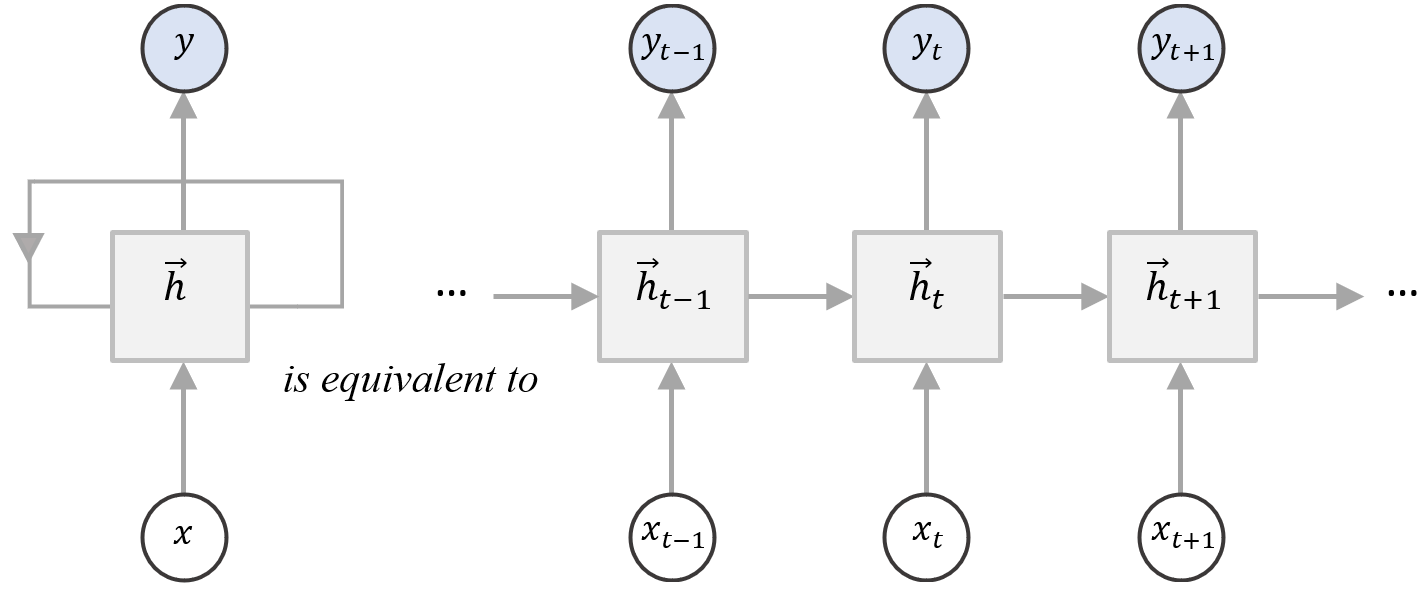
\includegraphics[width=1\textwidth]{Images/RNN_diagram1.png}\\
		\centering\textbf{Figure 6}: Illustration of RNN Cell
	\end{figure}
\end{minipage}\\\vspace{-10pt}

\noindent RNNs are limited to looking back only a few steps as they are susceptible to the \textit{vanishing gradient problem}, more so when we continue to add complexity (in the form of additional layers) to our network. RNNs use backpropagation to calculate the gradient of the loss function with respect to individual network weights, and these weights are updated in a manner that is proportional to the gradient. However, when the vanishing gradient problem occurs, the gradient with respect to the earliest layers becomes negligible; therefore the updates made to weights in these layers become insignificant. This can make the learning process slow and unstable, causing the network to have only a short-term memory.

Variations of the vanilla RNN such as \textit{Long Short-Term Memory (LSTM)} \cite{hochreiter1997long} and \textit{Gated Recurrent Units (GRU)}\cite{cho2014learning} use internal mechanisms, known as gates, which allow them to overcome the issue of short-term memory by controlling how much information is forgotten or allowed to pass through to the output. We implement an LSTM and GRU (as well as their bidirectional variants), comparing their performance against that of a standard RNN. Bidirectional models concatenate the output sequences of two recurrent layers, where one is trained on reversed input sequences and the other is trained on the original input sequences. This allows context to be captured from both directions, and can lead to improved predictions.

%A directed cycle is formed within an RNN whereby former outputs are input back into a hidden unit. This hidden state represents the context based on prior inputs, giving rise to the \textit{temporal dimension} in RNNs which allows them to take into account time and sequencing. This leads to the interesting property that the same input could produce a different output depending on the previous inputs given to the RNN.

%In a vanilla RNN, the input and hidden state are simply propagated through a single tanh layer. However in a Long Short Term Memory model (LSTM), three gates are introduced, as well as a cell state, allowing an LSTM to better preserve long-term dependencies. We implement a Vanilla RNN as a baseline against which to compare our more advanced RNN models, as well as three additional models as described below:

% RNNs have been successfully applied to language-related tasks. Often, we may require more context than just the most recent surrounding text. The gap between the most relevant information needed to form a prediction can be very wide, if the relevent contextual information was given at the beginning of the paragraph. LSTMs are especially suited to processing sequential, or time-series, information such as text. This is due to the fact that RNNs have a 'memory', in that the input to the current step is the output from the previous step. However, they suffer from the vanishing gradient problem. This is where gradient values get smaller as it backtracks through lower layers, making it harder for the network to update weights and causing calculations to take longer. Recurrent Neural Networks are not very good at remembering long term dependencies, therefore in this instance we can use \textit{Long short-term memory (LSTM)} models \cite{hochreiter1997long} instead which are more effective at preserving long term dependencies.

%\begin{enumerate}
	%\item \textbf{Gated Recurrent Unit -- } Introduced in Cho et al.\ (2014) \cite{cho2014learning}, GRUs use an update gate and a reset gate to determine how much information from earlier time steps needs to be passed to successive time steps and how much should be forgotten.
	
	%The reset gate is used to 
	
	%\item \textbf{Long Short-term Memory \textit{(LSTM)} -- } They use \textit{input}, \textit{output} and \textit{forget} gates 
	
	%three gates are introduced, as well as a cell state, allowing an LSTM to better preserve long-term dependencies
%\end{enumerate}

\subsection{Attention}
\vspace{-4.2pt}
\noindent When humans read text to answer a query or to inform a decision, we automatically focus more on specific regions, such as the text surrounding key words or phrases. This is known as \textit{human visual attention} and has been well studied by psychologists; however, it is possible to incorporate a similar attention mechanism into our recurrent deep learning models. The intuition behind this is such that not all components of text are equally relevant for indicating sarcasm or not sarcasm; hence, this provides insight into which tokens contribute more or less in classification decisions. Additionally, incorporating an attention mechnism can lead to better classification performance. Extending our binary classification solution in this way enables us to answer the research question: \textit{Can a custom model identify which linguistic cues correlate more to sarcastic labels?}\\\vspace{-5pt}

\noindent We employ the word-level attention layer outlined in Yang et al.\ (2016) \cite{yang2016hierarchical} which uses context to identify relevant tokens, rather than filtering for key words irrespective of their context. This is an intermediate layer placed after the bi-directional RNN layer in our solution, as our attention mechanism utilises the forward and backward outputs of this layer. For a given word, $w_{it}$, the forward and backward hidden states of the bi-directional RNN are concatenated to obtain a sequence, $h_{it}$. This annotation harnesses the contextual information of the tokens that come before and after $w_{it}$; crucial for informing classification decisions and producing meaningful attention visualisations, as words can have different meanings depending on the context in which they are found. Figure 7 shows the word-level attention mechanism used in this project. Three trainable weights, $W_w$, $b_w$ and $u_w$, are intialised from a random normal distribution.\vspace{-10pt}

\hspace{-17pt}\begin{minipage}{0.65\textwidth}
	 Each word annotation, $h_{it}$ is fed through a fully-connected layer with tanh activation to produce $u_{it}$ - this is the hidden representation of $h_{it}$ (1). We apply the softmax function to the similarity between a word-level context vector ($u_w$), learned during training, and $u_{it}$ (2). This produces an attention weight, $\alpha_{it}$, which represents the relative importance of the token $w_{it}$ in the sentence, s. Finally, the sentence-level context vector, $s_i$, is computed as the sum of $h_{it} \cdot a_{it}$ over all timesteps, t (3).
\end{minipage}
\hspace{2pt}
\begin{minipage}{0.35\textwidth}
\begin{figure}[H]
	\begin{center}
		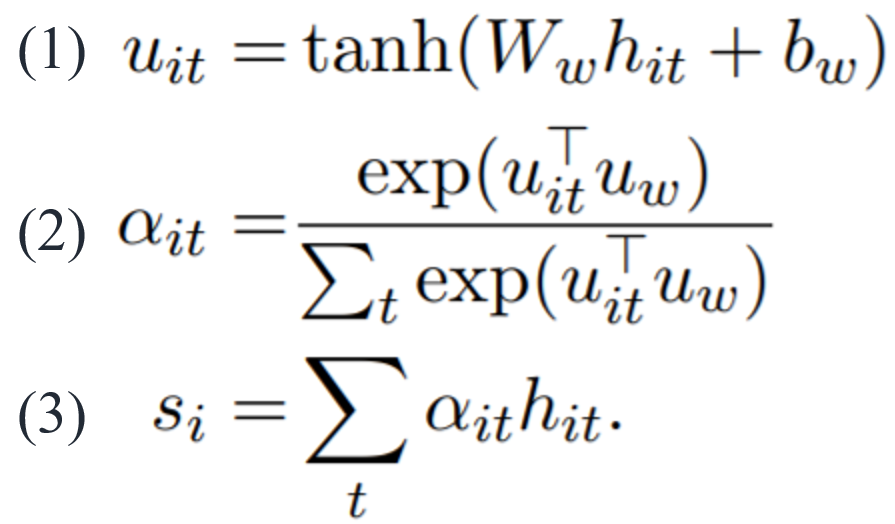
\includegraphics[width=0.95\textwidth]{Images/wordLevelAttention.png}\\
		\textbf{Figure 7:} Word-level attention mechanism\cite{yang2016hierarchical}\\
	\end{center}
\end{figure}
\end{minipage}

\noindent Our attention layer returns the attention weight, $a_{it}$ for each token, as well as the sentence-level content vector, $s_i$, which is propagated through the remainder of our classifier. We visualise our attention weights by projecting them into a colour-space and displaying the tokens highlighted in their respective colours, where darker colours indicate a higher-level of attention.

\section{Results}\vspace{-8pt}
\subsection{Evaluation Method}\vspace{-5pt}
\noindent This section discusses our approach to evaluating the performance of the trained models. Each trained model makes predictions on labelled unseen data, and these predictions are compared to the corresponding ground truth labels. From this, we extract the number of true positives (TP), true negatives (TN), false positives (FP) and false negatives (FN). We use four metrics that leverage this data differently to produce an evaluation of the trained models.\vspace{-10pt}

\hspace{-30pt}\begin{center}
	\begin{minipage}{0.47\textwidth}
		$Precision =\frac{TP}{TP\text{ } + \text{ }FP}$\\
	\end{minipage}
	\hspace{-30pt}\begin{minipage}{0.47\textwidth}
		$Recall =\frac{TP}{TP\text{ } + \text{ }FN}$\\
	\end{minipage}\\
\end{center}
\vspace{-20pt}
\begin{center}
	\begin{minipage}{0.47\textwidth}
		$F_1\text{ } Score =\frac{2 \text{ }\times\text{ } precision\text{ } \times \text{ }recall}{precision\text{ } + \text{ }recall}$
	\end{minipage}
	\hspace{-30pt}\begin{minipage}{0.47\textwidth}
		$MCC =\frac{TP \text{ } \times \text{ } TN \text{ } - \text{ } FP\text{ } \times \text{ } FN}{\sqrt{(TP \text{ } + \text{ } FP)(TP \text{ } + \text{ } FN)(TN \text{ } + \text{ } FP)(TN \text{ } + \text{ } FN)}}$
	\end{minipage}
\end{center}

\noindent Precision refers to the proportion of classified-sarcastic data that is \textit{truly sarcastic} (how many positives are true positives), and recall describes the proportion of the truly sarcastic data that is classified as such (how many true positives are labelled as positives). We also use the harmonic mean of precision and recall ($F_{1}$ score), however this metric has faced some criticism for giving equal weight to precision and recall \cite{hand2018note}, therefore we also consider these measures separately. The Matthews Correlation Co-efficient (MCC) is a balanced measure which shows high scores if the true positive and negative rates are high and if the false positive and negative rates are low.

%this section presents the results of the solutions.  It should include information on experimental settings.  The results should demonstrate the claimed benefits/disadvantages of the proposed solutions.
\subsection{Analysis of Sentiment Features}\vspace{-5pt}
\noindent We analyse the effectiveness of our novel sentiment features in comparison to our standard punctuation and topic modelling features by feeding them to logistic regression models and calculating the $F_1$ scores using 5-fold cross-validation; logistic regression is used as these feature vectors are small. We consider models achieving $F_1$ scores greater than 0.5 to be indicative of useful training features, as a binary classification model predicting randomly on a balanced dataset achieves an average score of 0.5. \\\vspace{-20pt}


\begin{center}
	\textbf{Table 4}: $F_1$ score of logistic regression models trained on hand-crafted features
\end{center}\vspace{-20pt}

\begin{center}
	\begin{tabular}{|c||c|c|c|} 
	\hline
	\textbf{Dataset} & \textbf{Sentiment} & \textbf{Punctuation} & \textbf{Topic} \\ [0.4ex] 
	\hline\hline
	News Headlines& 0.516 & 0.344 & 0.525\\ 
	\hline
	Twitter Data & 0.593 & 0.611 & 0.530\\
	\hline
\end{tabular}
\end{center}\vspace{-5pt}

\noindent All three features were more informative when extracted from Twitter data, and this may be due to the informal and irregular nature of user-generated tweets.\ Sarcasm in tweets is more overt than in News headlines, which are typically contextual and subtley sarcastic.\ This enables us to assess whether these features alone are indicative of sarcasm in different media types.\ Figure \_ illustrates the distributions of the overall sentiment labels (value 5 in our sentiment feature vectors) for both of our datasets.\ Sarcastic and non-sarcastic instances are represented separately, as differences in their distributions enable us to explain the classification scores in table \_.


\hspace{-30pt}
\begin{minipage}{0.3\textwidth}
\begin{figure}[H]
	\begin{center}
		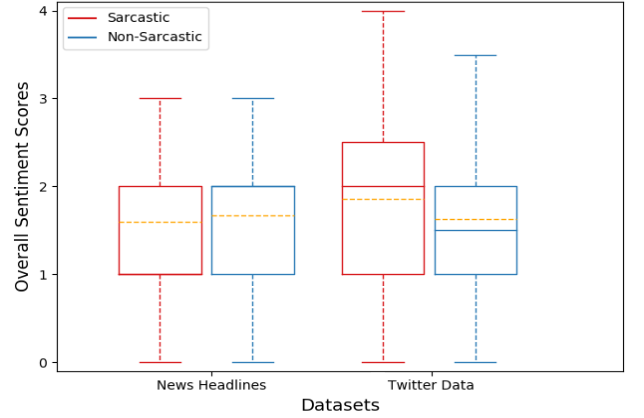
\includegraphics[width=1\textwidth]{Images/boxcompare.png}\\
		\textbf{Figure 8:} Visualisation of overall sentiment\\
	\end{center}
\end{figure}
\end{minipage}
\hspace{5pt}
\begin{minipage}{0.70\textwidth}
	
	
	
	For the Sarcasm Amazon Review Corpus, within most sentiment classes there is a greater difference in the proportion of tokens for non-sarcastic and sarcastic instances. This indicates that sarcastic and non-sarcastic instances are easier to distinguish, given that their sentiment compositions are more distinct. The News Headlines for Sarcasm Detection results displays the opposite, and this explains why the logistic regression classifier trained on this data achieved an $F_1$  score of only 0.515, as the features for each class are very similar.
\end{minipage}\vspace{-5pt}


%\noindent Our results show that sentiment features are indicative of sarcasm when extracted from the Sarcasm Amazon Review Corpus, however when extracted from the News Headlines for Sarcasm Detection, they were ineffective. To further examine this relationship between sarcasm and sentiment, we compute the mean proportion of tokens in each sentiment class for sarcastic and non-sarcastic instances. We then compute the absolute differences of these values between the sarcastic and non-sarcastic classes - the intuition being that it is simpler for a classifier to separate samples where there is a clearer distinction between the expected features of each class. Hence, where the absolute difference in the mean proportion of tokens between sarcasm classes is higher, a classifier is better able to correctly annotate samples. A visualisation of these results is given in the figure below.



\subsection{Binary Classification}\vspace{-5pt}
\noindent To compare the performance of our machine learning and deep learning classifiers, each model is trained independently on numerous features extracted from our datasets. For each dataset, we report on only a subset of our most informative results, including our highest-achieving models and those that produced unexpectedly good or bad results. We contrast the performance of our machine learning and deep learning classifiers in order to answer the research question: \textit{Do deep learning techniques perform better than machine learning approaches?}\\\vspace{-5pt}

%Hence, we curate a selection of models that either produce the best scores, or exceeded our expectations.


\noindent \textbf{Experimental Settings --} For our machine learning experimentation, 5-fold cross validation is employed to ensure reproducability and consistency of results. However, it is infeasible to apply the same approach to our deep learning experimentation, as training is substantially slower.\ We train each deep learning model on GloVe and ElMo vectors only, as it is computationally intractable to train neural networks on high-dimensional sparse features.\ The upper-bound on the number of training epochs is 300, although this is seldom reached due to the use of the \textit{Early Stopping} callback function. \vspace{-4pt}

\begin{enumerate}
	\item \textbf{Early stopping --} Training is interrupted when the validation loss stops declining - this is used to determine the appropriate number of epochs.\vspace{-8pt}
	\item \textbf{Model Checkpointing --} We track and save the weights of the best performing model during training i.e.\ the model with the lowest validation loss.
\end{enumerate}\vspace{-4pt}

\noindent Model performance peaks early in the training process for all of our models, although there is some fluctuation in the optimal number of epochs for different model types, hence early stopping is incorporated to stop training once model performance begins to plateau. The number of epochs for which no improvement in validation loss is seen (\textit{patience}) is set to 10. Setting the patience too low can hamper a model that plateaus for a while before improving again. We allocate 90\% of data to the training set, and the remaining 10\% to the testing set.

\subsubsection{News Headlines Dataset}
\begin{center}
	\textbf{Table 5}: Classification results on the \textit{News Headlines} dataset
\end{center}

\begin{center}
	\begin{tabular}{ |c||c|c|c|c|}
		\hline
		\textbf{Machine Learning Model}& \textbf{Feature(s)*} & \textbf{Precision} & \textbf{Recall} & \textbf{$\mathbf{F_1}$ Score}\\
		\hline\hline
		Random Forest Classifier & GloVe  & 0.774   & 0.735 & 0.754\\
		Support-Vector Machine & TF-IDF  & 0.688   & 0.751 & 0.718\\
		Random Forest Classifier & ElMo  & 0.801   & 0.793 & 0.797\\
		Logistic Regression & ElMo  & 0.840   & 0.852 & 0.846\\
		Logistic Regression & ElMo $\cdot$ S $\cdot$ T & \textbf{0.848}   & \textbf{0.854} & \textbf{0.851}\\
		\hline\hline
		\textbf{Deep Learning Model}& \textbf{Feature(s)} & \textbf{Precision} & \textbf{Recall} & \textbf{$\mathbf{F_1}$ Score}\\
		\hline
		CNN & GloVe  & 0.818 & 0.806 & 0.812\\
		LSTM & ElMo  & 0.843   & 0.878 & 0.860\\
		Bidirectional LSTM & GloVe  & 0.855   & 0.873 & 0.864\\
		Deep CNN & ElMo & 0.873   & 0.869 & 0.871\\
		Bidirectional GRU & ElMo  & \textbf{0.888}   & \textbf{0.901} & \textbf{0.875}\\
		\hline
	\end{tabular}
\end{center}
\textit{*S} refers to sentiment features and \textit{T} refers to topic features\\\vspace{-10pt}


Notes:
- comment on sentiment and topic features
- best-performing ML model had highest of all three metrics
- ElMo always performs better than the other three feature types across comparable models.
- TF-IDF features performed better than GloVe features on our support-vector machine, however use of Bag of Words consistently led to the lowest scores across this dataset.
- 


\noindent Deep learning models routinely outperform Machine learning models.
Logistic regression trained on ElMo with sentiment and topic features was the machine learning model with the highest $F_1$ score, and a slight improvement of 0.1\%. The Random Forest Classifier was the next best model architecture on this dataset, although its $F_1$ score was 5.9\% lower than the best performing model. 

Our advanced RNN models exceeded the $F_1$ score of the vanilla RNN by an average of \_\%, which achieved an $F_1$ score of \_. Similarly, our deep CNN achieved an 8.2\% increase in $F_1$ score compared to our simple CNN, as well as more consistent values for precision and recall.

\subsubsection{Twitter Dataset}

\begin{center}
	\textbf{Table 6}: Classification results on the \textit{Twitter} dataset
\end{center}

\begin{center}
	\begin{tabular}{ |c||c|c|c|c|}
		\hline
		\textbf{Machine Learning Model}& \textbf{Feature(s)*} & \textbf{Precision} & \textbf{Recall} & \textbf{$\mathbf{F_1}$ Score}\\
		\hline\hline
		Gaussian Na\"{i}ve Bayes & Bag of Words & 0.677 & 0.685 & 0.681\\
		Random Forest Classifier & GloVe  & 0.669   & 0.623 & 0.645\\
		Support-Vector Machine & ElMo  & 0.722 & \textbf{0.789} & 0.754\\
		Logistic Regression & ElMo  & 0.758 & 0.766 & 0.762\\
		Logistic Regression & ElMo $\cdot$ S $\cdot$ T $\cdot$ P & \textbf{0.794} & 0.786 & \textbf{0.790}\\
		\hline\hline
		\textbf{Deep Learning Model}& \textbf{Feature(s)} & \textbf{Precision} & \textbf{Recall} & \textbf{$\mathbf{F_1}$ Score}\\
		\hline
		Vanilla RNN & ElMo  & 0.834   & 0.801 & 0.817\\
		Bidirectional LSTM & GloVe  & 0.829 & 0.815 & 0.822\\
		CNN & ElMo  & \textbf{0.851}   & 0.814 & 0.832\\
		Bidirectional LSTM & ElMo  & 0.847   & \textbf{0.851} & \textbf{0.849}\\
		Long Short-Term Memory & GloVe & 0.837   & 0.845 & 0.841\\
		\hline
	\end{tabular}
\end{center}
\textit{*S} refers to sentiment features, \textit{T} refers to topic features and \textit{P} refers to punctuation features\\

\noindent As the best-performing machine learning model trained on GloVe vectors, the Random Forest classifier attained an $F_1$ score of 0.645 - 15.4\% lower than our logistic regression model trained exclusively on ElMo vectors. Models trained on GloVe vectors showed poor performance on this particular dataset, and this could be due to the fact that this dataset has the lowest percentage of tokens present in the GloVe dictionary; hence, we lose the meaning of these tokens in the input embeddings.




\subsubsection{Cross-Dataset Evaluation}
Given that the Bidirectional LSTM and Bidirectional GRU achieved the highest $F_1$ scores on the Twitter and News Headlines dataset, respectively. It is crucial to the success of our solution that these models are able to generalise to other forms of media, hence we assess our candidate solutions on an evaluation dataset of 1254 Amazon reviews. This gives us an indication of which model is more likely to generalise to unseen data in multiple forms of media (i.e. which model is most adaptable, therefore the most suitable to be used in our tool).

\begin{minipage}{0.4\textwidth}
	\begin{figure}[H]
		\begin{center}
			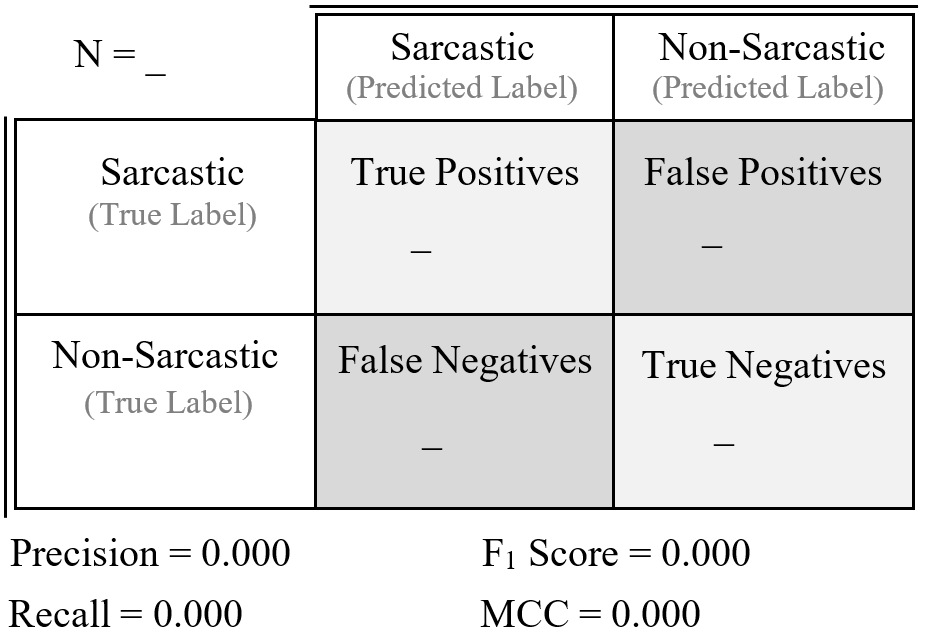
\includegraphics[width=0.75\textwidth]{Images/cm2.png}\\
			(a) Trained on News Headlines\\
		\end{center}
	\end{figure}
\end{minipage}
\begin{minipage}{0.4\textwidth}
	\begin{figure}[H]
		\begin{center}
			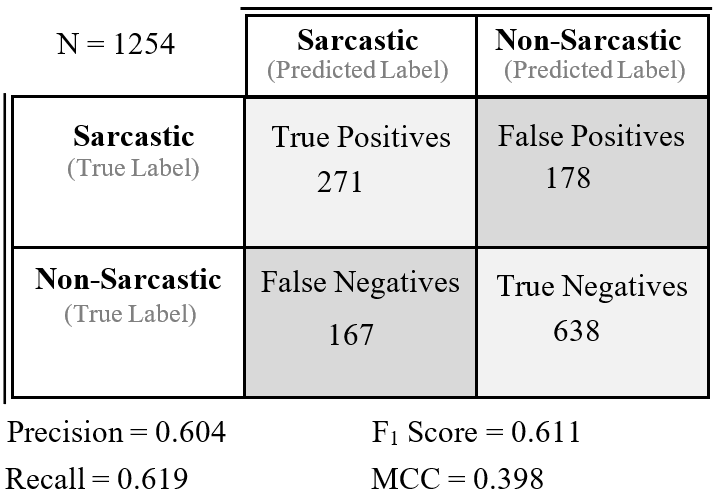
\includegraphics[width=0.75\textwidth]{Images/cm1.png}\\
			(b) Trained on Twitter Data\\
		\end{center}
	\end{figure}
\end{minipage}\vspace{-15pt}

\begin{center}
	\textbf{Figure 9}: Confusion Matrices of models evaluated on Amazon Reviews
\end{center}

\noindent False positives and negatives make up 44.7\% of our results for the News Headlines model, compared with 27.5\% on the Twitter model. This is reflected in the summary statistics produced for each model, as all metrics demonstrated better performance for our Twitter Model. 

The Matthews Correlation Coefficient is weaker for our Twitter model,

\subsection{Attention}\vspace{-5pt}
\noindent The superior model in the binary classification task is shown to be the Bidirectional LSTM model, trained on ElMo vectors from the Twitter dataset. We incorporate our attention mechanism after our bidirectional LSTM layer to identify the tokens that lead to positive and negative classification decisions. We present a number of attention visualisations, and examine whether incorporating attention can boost model performance as hypothesised, and for what training cost.\\\vspace{-5pt}


\hspace{-5pt}\begin{minipage}{0.5\textwidth}
	\vspace{2pt}\begin{minipage}{0.48\textwidth}
		\begin{center}
			\hspace{-1cm}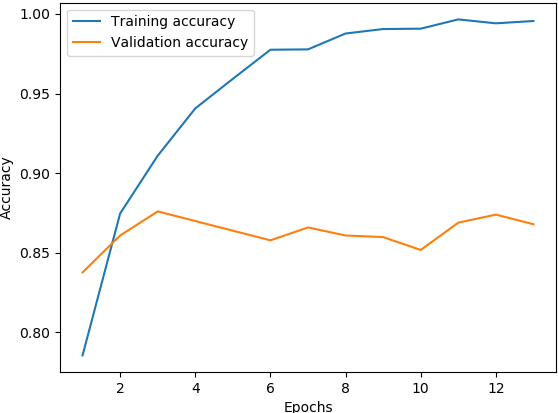
\includegraphics[width=1\textwidth]{Images/lstm.png}\\
			\hspace{-1cm}\textbf{(a)} Without Attention\\
		\end{center}
	\end{minipage}
	\vspace{2pt}\begin{minipage}{0.48\textwidth}
		\begin{center}
			\hspace{-1cm}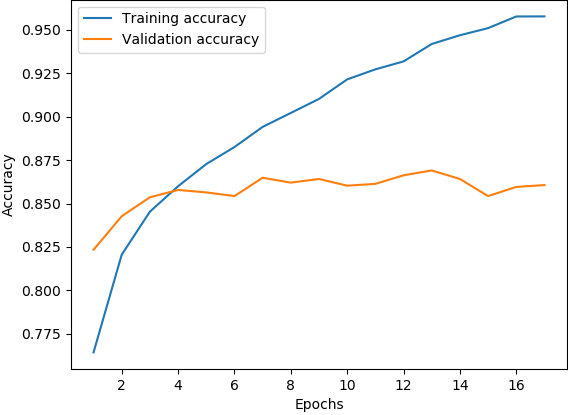
\includegraphics[width=1\textwidth]{Images/attention-lstm.png}\\
			\hspace{-1cm}\textbf{(b)} With Attention\\
		\end{center}
	\end{minipage}
	\vspace{-5pt}\begin{center}
		\hspace{-20pt}\textbf{Figure 10:} Fluctuation of training and validation accuracy of models during training\\
	\end{center}
\end{minipage}
\hspace{-10pt}
\begin{minipage}{0.5\textwidth}
	\begin{center}
		\textbf{Table 7}: Comparison of bidirectional LSTM classification results\vspace{5pt}
		\begin{tabular}{|p{1.6cm}||p{1.8cm}|p{2cm}|}
			\hline
			& \multicolumn{2}{c|}{Bidirectional LSTM} \\
			\hline
			Metrics & With Attention & Without Attention\\
			\hline\hline
			Precision & 0.859 & 0.847\\
			\hline
			Recall & 0.865 & 0.851\\
			\hline
			$F_1$ Score & 0.862 & 0.849\\
			\hline
		\end{tabular}
	\end{center}	
\end{minipage}\vspace{10pt}

\noindent Incorporating our attention mechanism led to an increase in training time as the number of training epochs increased from 12 to 16 (\textit{figure 10}). Furthermore, the validation accuracy increased at a steadier rate and peaked at a slightly lower value than in our non-attention model. However, the performance of our bidirectional LSTM with attention mechanism exceeds our foremost solution in the binary classification task, improving upon precision, recall and $F_1$ score by an average of 1.51\% \textit{(table 7)}.\\

\hspace{-5pt}\begin{minipage}{0.5\textwidth}
	\begin{center}
		\hspace{-1cm}
\includegraphics[width=1\textwidth]{Images/visualisation1.png}\\
		\hspace{-1cm}\textbf{(a)} Without Attention\\
	\end{center}
\end{minipage}
\hspace{-10pt}
\begin{minipage}{0.5\textwidth}
	\begin{center}
		\hspace{-1cm}
\includegraphics[width=1\textwidth]{Images/visualisation2.png}\\
		\hspace{-1cm}\textbf{(a)} Without Attention\\
	\end{center}	
\end{minipage}

%As such, we incorporate an ElMo embedding layer to produce contextualised word embeddings from raw text, as they encode the context in which a word is found (polysemy) and can generalise to out-of-vocabulary tokens. We feed these word embeddings through a bidirectional long short-term memory model in order to retain both the left and right contexts of each word.\\


\noindent Visualising the output of our attention layer shows that the model places more emphasis on qualitatively informative tokens.


\section{Evaluation}
\noindent In the following section, we analyse the effectiveness of the solution, discussing its strengths and weaknesses and evaluating to what extent it satisfies the research questions and deliverables.


News headlines are written formally, hence there is little noise in this dataset due to the absence of erroneous spelling. These headlines are self-contained, unlike tweets which may be in response to another tweet thereby excluding necessary context.

These reviews are typically longer than the average tweet, which is capped at 280 characters. The author's punctuation and spelling is preserved, therefore this data is very messy. This is the smallest of the three datasets. 

Hence, some of the sarcastic instances may not be sarcastic, and some non-sarcastic instances may be sarcastic.

\subsection{Solution Strengths}\vspace{-10pt}
\noindent We found that sentiment features are objectively useful predictors of sarcasm in Twitter data and News Headlines, as logistic regression models trained on these features achieved $F_1$ scores of 0.593 and 0.516, respectively. We found that sentiment features were most informative when extracted from Twitter data as opposed to News Headlines, and we hypothesise that this is due to the use of more overtly sarcastic expressions that utilise strong sentiment, such as "\textit{i love working weekends! \#not}". As both models achieved $F_1$ scores exceeding 0.5, this indicates that their performance bettered that of a trivial classifier which predicts class labels with apparent randomness. Hence, we conclude that sentiment features are sufficiently informative so as to guide a model to make non-trivial predictions.

We demonstrated the powerful capabilities of deep-learning architectures, as well as the potential for some machine learning models to compete with less sophisticated deep neural architectures when trained for a fraction of the time. For example, we achieved an $F_1$ score of 0.851 using a logistic regression model, trained with state-of-the-art contextualised word embeddings and hand-crafted sentiment and topic features.

We integrate an Attention layer into a bidirectional GRU and incorporate a mechanism for visualising the attention weights in order to highlight the tokens correlating more to sarcastic and non-sarcastic labels.\\

% use word exemplary

\noindent The \textbf{research questions} guiding this project are as follows --\\
\indent \textit{- Can handcrafted sentiment features improve sarcasm predictions?}\\ 
\indent \textit{- Do deep learning techniques perform better than machine learning approaches?}\\ 
\indent \textit{- Can a custom model identify which linguistic cues correlate more to sarcastic labels?}\\





\subsection{Solution Limitations}\vspace{-10pt}
It was only feasible to evaluate a small range of online media types, however surveying a broader range of media types could give us a wider perspective of sarcasm in online media.
Can handcrafted sentiment features improve sarcasm predictions?

Our deep learning architectures do not explicitly consider sentiment as a predictor of sarcasm.

However, there is evidence to suggest that sentiment features 
are no more informative than conventional lexical features - two key findings were noted. Firstly,  

; however, sentiment features extracted from News Headlines showed poor performance in comparison. 

\textit{some} forms of media. This may be due to the fact that sarcasm must be more overt in product reviews in order to mock the product, rather than the subtle, more contextualised instances in News Headlines.


\subsection{Lessons learnt}\vspace{-10pt}
We learned that 


\subsection{Project organisation and approach}\vspace{-10pt}




%This section should between 1 to 2 pages in length.

\section{Conclusions}
In terms of satisfying the objectives, this project was an overall success. With an interactive console, it may be useful to individuals who struggle to detect sarcasm in their daily-life, or for the industrial applications of enhanced opinion mining.

The main contributions of this project are as follows: sentiment features are combined with state-of-the-art vectorisation approaches. 

For future work, it would be interesting to explore the use of sarcasm in a wider variety of media types, and to extend support to additional non-English languages. Exploring the use of transfer learning with Transformers (BERT) may also produce interesting results.


%This section summarises the main points of this paper.  Do not replicate the abstract as the conclusion.  A conclusion might elaborate on the importance of the work or suggest applications and extensions.  This section should be no more than 1 page in length.

%The page lengths given for each section are indicative and will vary from project to project but should not exceed the upper limit.  A summary is shown in Table \ref{summary}.

%\begin{table}[htb]
%\centering
%\caption{SUMMARY OF PAGE LENGTHS FOR SECTIONS}
%\vspace*{6pt}
%\label{summary}
%\begin{tabular}{|ll|c|} \hline
%& \multicolumn{1}{c|}{\bf Section} & {\bf Number of Pages} \\ \hline
%I. & Introduction & 2--3 \\ \hline
%II. & Related Work & 2--3 \\ \hline
%III. & Solution & 4--7 \\ \hline
%IV. & Results & 2--3 \\ \hline
%V. & Evaluation & 1-2 \\ \hline
%VI. & Conclusions & 1 \\ \hline
%\end{tabular}
%\end{table}


\bibliography{FinalPaper}


\end{document}